%--------------------------------------
%CANEVAS
%--------------------------------------

%utiliser les environnement \begin{comment} \end{comment} pour mettre en commentaire le préambule une fois la programmation appelée dans le document maître (!ne pas oublier de mettre en commentaire \end{document}!)

\begin{comment}

\documentclass[a4paper, 11pt, twoside, fleqn]{memoir}

\usepackage{AOCDTF}

\marqueurchapitre
\decoupagechapitre{1} %juste pour éviter les erreurs lors de la compilation des sous-programmations (passera en commentaire)

%lien d'édition des figures Tikz sur le site mathcha.io (rajouter le lien d'une modification effectuée sur la figure tikz avec le nom du modificateur car il n'y a qu'un lien par compte)

%lien mathcha Nom Prénom : https://www.mathcha.io/editor/ml76PuOwsvWh8WD77ytO3OJn2Hlvq8GNF3g2Jwd

%--------------------------------------
%corps du document
%--------------------------------------

\begin{document} %corps du document
	\openleft %début de chapitre à gauche

\end{comment}


\begin{figure}[H]
\caption{Structure matérielle d'un système automatisé}
\tikzset{every picture/.style={line width=0.75pt}} %set default line width to 0.75pt        

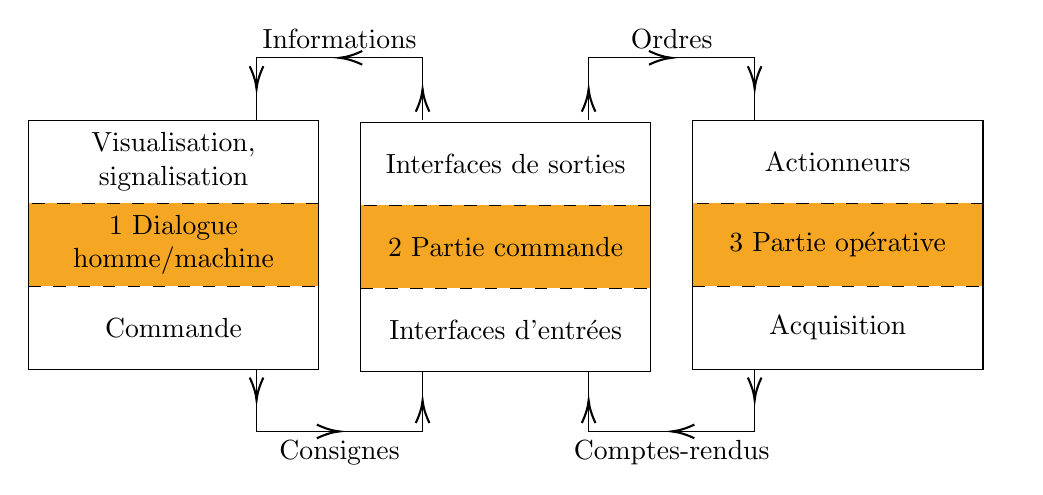
\begin{tikzpicture}[x=0.75pt,y=0.75pt,yscale=-1,xscale=1]
%uncomment if require: \path (0,300); %set diagram left start at 0, and has height of 300

%Shape: Rectangle [id:dp10260270003045247] 
\draw  [fill={rgb, 255:red, 245; green, 166; blue, 35 }  ,fill opacity=1 ] (100,90) -- (240,90) -- (240,210) -- (100,210) -- cycle ;
%Shape: Rectangle [id:dp6595603315617775] 
\draw  [fill={rgb, 255:red, 255; green, 255; blue, 255 }  ,fill opacity=1 ][dash pattern={on 4.5pt off 4.5pt}] (100,90) -- (240,90) -- (240,130) -- (100,130) -- cycle ;
%Shape: Rectangle [id:dp9769956373140513] 
\draw  [fill={rgb, 255:red, 255; green, 255; blue, 255 }  ,fill opacity=1 ][dash pattern={on 4.5pt off 4.5pt}] (100,170) -- (240,170) -- (240,210) -- (100,210) -- cycle ;
%Shape: Rectangle [id:dp5049152868754619] 
\draw  [fill={rgb, 255:red, 245; green, 166; blue, 35 }  ,fill opacity=1 ] (260,91) -- (400,91) -- (400,211) -- (260,211) -- cycle ;
%Shape: Rectangle [id:dp9221854973091113] 
\draw  [fill={rgb, 255:red, 245; green, 166; blue, 35 }  ,fill opacity=1 ] (420,90) -- (560,90) -- (560,210) -- (420,210) -- cycle ;
%Straight Lines [id:da1386624660715703] 
\draw    (210,90) -- (210,60) -- (290,60) -- (290,90) ;
\draw [shift={(210,75)}, rotate = 270] [color={rgb, 255:red, 0; green, 0; blue, 0 }  ][line width=0.75]    (10.93,-3.29) .. controls (6.95,-1.4) and (3.31,-0.3) .. (0,0) .. controls (3.31,0.3) and (6.95,1.4) .. (10.93,3.29)   ;
\draw [shift={(250,60)}, rotate = 0] [color={rgb, 255:red, 0; green, 0; blue, 0 }  ][line width=0.75]    (10.93,-3.29) .. controls (6.95,-1.4) and (3.31,-0.3) .. (0,0) .. controls (3.31,0.3) and (6.95,1.4) .. (10.93,3.29)   ;
\draw [shift={(290,75)}, rotate = 90] [color={rgb, 255:red, 0; green, 0; blue, 0 }  ][line width=0.75]    (10.93,-3.29) .. controls (6.95,-1.4) and (3.31,-0.3) .. (0,0) .. controls (3.31,0.3) and (6.95,1.4) .. (10.93,3.29)   ;
%Straight Lines [id:da24586017428466933] 
\draw    (210,210) -- (210,240) -- (290,240) -- (290,210) ;
\draw [shift={(210,225)}, rotate = 270] [color={rgb, 255:red, 0; green, 0; blue, 0 }  ][line width=0.75]    (10.93,-3.29) .. controls (6.95,-1.4) and (3.31,-0.3) .. (0,0) .. controls (3.31,0.3) and (6.95,1.4) .. (10.93,3.29)   ;
\draw [shift={(250,240)}, rotate = 180] [color={rgb, 255:red, 0; green, 0; blue, 0 }  ][line width=0.75]    (10.93,-3.29) .. controls (6.95,-1.4) and (3.31,-0.3) .. (0,0) .. controls (3.31,0.3) and (6.95,1.4) .. (10.93,3.29)   ;
\draw [shift={(290,225)}, rotate = 450] [color={rgb, 255:red, 0; green, 0; blue, 0 }  ][line width=0.75]    (10.93,-3.29) .. controls (6.95,-1.4) and (3.31,-0.3) .. (0,0) .. controls (3.31,0.3) and (6.95,1.4) .. (10.93,3.29)   ;
%Straight Lines [id:da47558842927164535] 
\draw    (370,90) -- (370,60) -- (450,60) -- (450,90) ;
\draw [shift={(370,75)}, rotate = 450] [color={rgb, 255:red, 0; green, 0; blue, 0 }  ][line width=0.75]    (10.93,-3.29) .. controls (6.95,-1.4) and (3.31,-0.3) .. (0,0) .. controls (3.31,0.3) and (6.95,1.4) .. (10.93,3.29)   ;
\draw [shift={(410,60)}, rotate = 180] [color={rgb, 255:red, 0; green, 0; blue, 0 }  ][line width=0.75]    (10.93,-3.29) .. controls (6.95,-1.4) and (3.31,-0.3) .. (0,0) .. controls (3.31,0.3) and (6.95,1.4) .. (10.93,3.29)   ;
\draw [shift={(450,75)}, rotate = 270] [color={rgb, 255:red, 0; green, 0; blue, 0 }  ][line width=0.75]    (10.93,-3.29) .. controls (6.95,-1.4) and (3.31,-0.3) .. (0,0) .. controls (3.31,0.3) and (6.95,1.4) .. (10.93,3.29)   ;
%Straight Lines [id:da04414261859625401] 
\draw    (370,210) -- (370,240) -- (450,240) -- (450,210) ;
\draw [shift={(370,225)}, rotate = 90] [color={rgb, 255:red, 0; green, 0; blue, 0 }  ][line width=0.75]    (10.93,-3.29) .. controls (6.95,-1.4) and (3.31,-0.3) .. (0,0) .. controls (3.31,0.3) and (6.95,1.4) .. (10.93,3.29)   ;
\draw [shift={(410,240)}, rotate = 0] [color={rgb, 255:red, 0; green, 0; blue, 0 }  ][line width=0.75]    (10.93,-3.29) .. controls (6.95,-1.4) and (3.31,-0.3) .. (0,0) .. controls (3.31,0.3) and (6.95,1.4) .. (10.93,3.29)   ;
\draw [shift={(450,225)}, rotate = 270] [color={rgb, 255:red, 0; green, 0; blue, 0 }  ][line width=0.75]    (10.93,-3.29) .. controls (6.95,-1.4) and (3.31,-0.3) .. (0,0) .. controls (3.31,0.3) and (6.95,1.4) .. (10.93,3.29)   ;
%Shape: Rectangle [id:dp23929095996485295] 
\draw  [fill={rgb, 255:red, 255; green, 255; blue, 255 }  ,fill opacity=1 ][dash pattern={on 4.5pt off 4.5pt}] (260,91) -- (400,91) -- (400,131) -- (260,131) -- cycle ;
%Shape: Rectangle [id:dp2763405581796431] 
\draw  [fill={rgb, 255:red, 255; green, 255; blue, 255 }  ,fill opacity=1 ][dash pattern={on 4.5pt off 4.5pt}] (260,171) -- (400,171) -- (400,211) -- (260,211) -- cycle ;
%Shape: Rectangle [id:dp7537953936366432] 
\draw  [fill={rgb, 255:red, 255; green, 255; blue, 255 }  ,fill opacity=1 ][dash pattern={on 4.5pt off 4.5pt}] (420,90) -- (560,90) -- (560,130) -- (420,130) -- cycle ;
%Shape: Rectangle [id:dp8221584429330733] 
\draw  [fill={rgb, 255:red, 255; green, 255; blue, 255 }  ,fill opacity=1 ][dash pattern={on 4.5pt off 4.5pt}] (420,170) -- (560,170) -- (560,210) -- (420,210) -- cycle ;
%Shape: Rectangle [id:dp7256077006177953] 
\draw   (100,90) -- (240,90) -- (240,210) -- (100,210) -- cycle ;
%Shape: Rectangle [id:dp09975149655953441] 
\draw   (260,91) -- (400,91) -- (400,211) -- (260,211) -- cycle ;
%Shape: Rectangle [id:dp8308335059986585] 
\draw   (420,90) -- (560,90) -- (560,210) -- (420,210) -- cycle ;

% Text Node
\draw (170,110) node   [align=left] {\begin{minipage}[lt]{65.47125pt}\setlength\topsep{0pt}
\begin{center}
Visualisation, \\signalisation
\end{center}

\end{minipage}};
% Text Node
\draw (170,150) node   [align=left] {\begin{minipage}[lt]{92.88375pt}\setlength\topsep{0pt}
\begin{center}
\Circled{1} Dialogue \\homme/machine
\end{center}

\end{minipage}};
% Text Node
\draw (170,190) node   [align=left] {\begin{minipage}[lt]{55.451875pt}\setlength\topsep{0pt}
\begin{center}
Commande
\end{center}

\end{minipage}};
% Text Node
\draw (330,111) node   [align=left] {\begin{minipage}[lt]{94.573125pt}\setlength\topsep{0pt}
\begin{center}
Interfaces de sorties
\end{center}

\end{minipage}};
% Text Node
\draw (330,151) node   [align=left] {\begin{minipage}[lt]{129.720625pt}\setlength\topsep{0pt}
\begin{center}
\Circled{2} Partie commande
\end{center}

\end{minipage}};
% Text Node
\draw (330,191) node   [align=left] {\begin{minipage}[lt]{91.99125000000001pt}\setlength\topsep{0pt}
\begin{center}
Interfaces d'entrées
\end{center}

\end{minipage}};
% Text Node
\draw (490,110) node   [align=left] {\begin{minipage}[lt]{56.588750000000005pt}\setlength\topsep{0pt}
\begin{center}
Actionneurs
\end{center}

\end{minipage}};
% Text Node
\draw (490,150) node   [align=left] {\begin{minipage}[lt]{121.22062500000001pt}\setlength\topsep{0pt}
\begin{center}
\Circled{3} Partie opérative
\end{center}

\end{minipage}};
% Text Node
\draw (490,190) node   [align=left] {\begin{minipage}[lt]{52.051875pt}\setlength\topsep{0pt}
\begin{center}
Acquisition
\end{center}

\end{minipage}};
% Text Node
\draw (250,57) node [anchor=south] [inner sep=0.75pt]   [align=left] {Informations};
% Text Node
\draw (410,57) node [anchor=south] [inner sep=0.75pt]   [align=left] {Ordres};
% Text Node
\draw (410,243) node [anchor=north] [inner sep=0.75pt]   [align=left] {Comptes-rendus};
% Text Node
\draw (250,243) node [anchor=north] [inner sep=0.75pt]   [align=left] {Consignes};


\end{tikzpicture}
\end{figure}
%\end{document}

